\documentclass{upmassignment}
\usepackage[spanish]{babel}
\usepackage{ifthen}
\usepackage{amsmath}
\usepackage{amsfonts}

%% PGFPLOTS %%
\usepackage{pgfplots}

%% TIKZ %%
\usepackage{tikz}
\usetikzlibrary{babel}
\usepackage{animate}
\usetikzlibrary{positioning}
\usetikzlibrary{shapes,arrows, positioning, calc}
\usetikzlibrary{overlay-beamer-styles}
\usetikzlibrary{chains,shapes.multipart}
\usetikzlibrary{scopes}
\usetikzlibrary{automata}
\usetikzlibrary{positioning}  %                 ...positioning nodes
\usetikzlibrary{arrows}       %                 ...customizing arrows
\usetikzlibrary{intersections}


% Para mostrar/ocultar soluciones
\newboolean{show}
\setboolean{show}{true}
%\setboolean{show}{false}
\usepackage{environ}
\NewEnviron{solucion}{
  \ifshow
      \begin{answer}\BODY\end{answer}
  \fi}


%% MATH commands
\DeclareMathOperator{\Var}{Var}




\coursetitle{Creating assignments}
\courselabel{RSTC}
\exercisesheet{Ejercicio de Alumno}{Temas 6 y 7}
\student{\ }%
\semester{Segundo Semestre}
\date{\today}
\university{Universidad Politécnica de Madrid}
\school{Departamento de Ingeniería de Sistemas Telemáticos}
%\usepackage[pdftex]{graphicx}
%\usepackage{subfigure}


\setlength{\textwidth}{5.0in}
\linespread{1.3}
\renewcommand{\PB}{{\bfseries Problema}}















\begin{document}

Se pretende modelar qué va a suceder en
el próximo Gran Premio de F1 de
Emilia-Romagna --
\textit{Autodromo Enzo e Dino Ferrari}.

\vspace{1em}

\begin{minipage}{\textwidth}
    \centering
    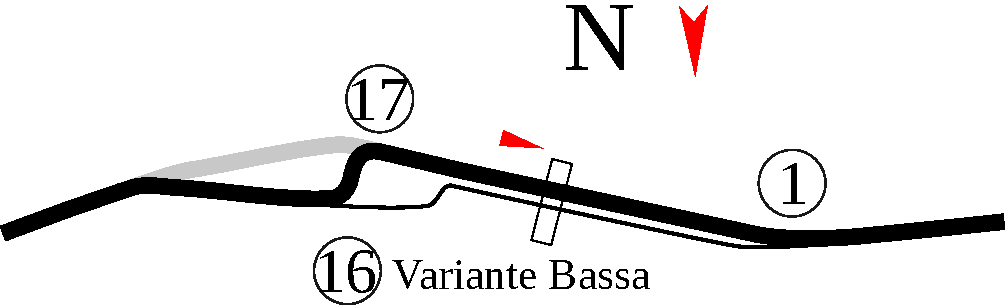
\includegraphics[width=.32\textwidth]{figs/box-pitlane.pdf}
\end{minipage}

\begin{problemlist}
    \pbitem El acceso a boxes tiene
    200 [m], un carril
    límite de velocidad de
    80 [km/h], y el tiempo de llegada
    entre coches es exponencial de media
    10~[sec]. ¿Cuál será entonces el tiempo
    medio de acceso a boxes?

    \begin{solucion}
        Primero, vemos que el tiempo entre llegadas
de coches
tiene media $\mathbb{E}[t_l]=\tfrac{1}{\lambda}=5$~[sec];
o dicho de otro modo, los coches llegan
a tasa $\lambda=\tfrac{1}{5}$~[coches/sec].

El tiempo que se tarda en acceder a boxes es
$t_s=\tfrac{200\cdot10^{-3}}{80}=\tfrac{5}{2}\cdot10^{-3}$~[h].
O lo que es lo mismo
$t_s=0.9$~[sec], y la tasa a la que
se accede a boxes es
$\mu=\tfrac{1}{t_s}=\tfrac{10}{9}$~[coches/sec].

Por tanto, tenemos un sistema M/G/1 en el que
el tiempo de servicio $t_s$ es determinista.
Usando la fórmula de Pollazceck-Khintchine
tenemos que el tiempo medio de tener que
esperar para entrar en boxes es
\begin{equation*}
    \mathbb{E}[W(t)]
    =\frac{\mathbb{E}[t_s^2]}{2(1-\rho)}
    =\frac{\mathbb{E}^2[t_s]+\Var[t_s]}{2(1-\rho)}
    =\frac{t_s^2+0}{2(1-\rho)}
\end{equation*}
que sustituyendo por
$\rho=\tfrac{\lambda}{\mu}=\tfrac{9}{50}$
nos da
\begin{equation*}
    \mathbb{E}[W(t)]=
    \frac{0.9^2}{2\left(1-\frac{9}{50}\right)}
    \simeq0.49~\text{[sec]}
\end{equation*}

Por tanto el tiempo medio de acceso a boxes es
\begin{equation*}
    \mathbb{E}[T(t)] = \mathbb{E}[W(t)]+
    \mathbb{E}[t_s]
    = 0.49 + 0.9 = 1.39~\text{[sec]}
\end{equation*}



    \end{solucion}


    \pbitem Verstappen (VER)
    y Pérez (PER) se han parado en pista.

    \vspace{1em}
    \begin{tikzpicture}[scale=0.7, every node/.style={scale=0.8}]
        \draw (0,0) -- (10,0);
        \draw (0,2) -- (10,2);
        \draw[dashed] (0,1) --
            (6.7,1);
        \draw[dashed] (7.3,1) -- (10,1);

        % RB cars
        \node[rectangle,draw,rotate=20] at
            (2,1.5) {PER};
        \node[rectangle,draw,rotate=70] at
            (7,1.2) {VER};

        \draw [->,thick] (0.2,1.5) to[out=-45,in=180] (2,.5) to[out=0,in=180] (10.5,0.2)
            node[rectangle,draw,
            anchor=west]
            {ALO};

    \end{tikzpicture}
    \vspace{1em}

    El resto de pilotos 
    tardan, en media, un tiempo exponencial de
    0.5~[sec] en cruzar a PER, y 1~[sec] en
    cruzar a VER. Como el
    tiempo entre pilotos es una
    exponencial de media 2~[sec], ¿cuánto
    tiempo tardan, en media, en pasar a
    PER y VER?

    \begin{solucion}
        Al pasar de largo cada piloto se puede formar
una cola. Por tanto para pasar a PER y a VER
hay que atravesar dos colas.

Tenemos que los tiempos entre llegadas de
pilotos es exponencial con tasa
$\lambda=(\mathbb{E}[t_l])^{-1}
=\tfrac{1}{2}$~[coches/sec]; y el tiempo en
cruzar a cada piloto es una v.a. exponencial
de tasa $\mu_{PER}=2$~[coche/sec] y
$\mu_{VER}=1$~[coche/sec].
Por tanto tenemos dos colas M/M/1 en fila:


\usetikzlibrary{calc}

\vspace{1em}
\begin{minipage}{\textwidth}
\centering
\begin{tikzpicture}
    % the rectangular shape with vertical lines
    \node[rectangle split, rectangle split parts=6,
    draw, rectangle split horizontal,
    text height=1cm,text depth=0.5cm,inner ysep=0pt] (wa) {};
    \fill[white] ([xshift=-\pgflinewidth,yshift=-\pgflinewidth]wa.north west) rectangle ([xshift=-15pt,yshift=\pgflinewidth]wa.south);
    
    % the circle
    \node[draw,circle,minimum size=1.5cm,anchor=west] (se) at (wa.east) {$\mu_{PER}$};
    
    % the arrows and labels
    \draw[->] (se.east) -- +(20pt,0) node (seEnd) {};
    \draw[<-] (wa.west) -- +(-20pt,0) node[left] {$\lambda$};
    
    
    
    
    %%%%%%%%%%%%%%%%%%%
    %%% Second queue
    %%%%%%%%%%%%%%%%%%%
    
    % the rectangular shape with vertical lines
    \node[rectangle split, rectangle split parts=6,
        draw, rectangle split horizontal,text height=1cm,text depth=0.5cm,inner ysep=0pt,anchor=west] (wa2) at (seEnd.east) {};
    \fill[white] ([xshift=-\pgflinewidth,yshift=-\pgflinewidth]wa2.north west) rectangle ([xshift=-15pt,yshift=\pgflinewidth]wa2.south);
    
    % the circle
    \node[draw,circle,minimum size=1.5cm,anchor=west] (se2) at (wa2.east) {$\mu_{VER}$};
    
    % the arrows and labels
    \draw[->] (se2.east) -- +(20pt,0) node (seEnd2) {};

    \node[anchor=south] at (seEnd.north west) {$\lambda_{VER}$};
\end{tikzpicture}
\end{minipage}
\vspace{1em}

Se puede ver que estas dos colas M/M/1
son una red de Jackson, y por tanto sabemos
que el tiempo medio en pasar a PER y VER es
\begin{equation*}
    \mathbb{E}[T(t)]=
    \frac{1}{\mu_{PER}-\lambda}
    +\frac{1}{\mu_{VER}-\lambda_{VER}}
    = \frac{1}{2-\frac{1}{2}}
    + \frac{1}{1-\frac{1}{2}}
    =\frac{2}{3}+2 = \frac{8}{3}~\text{[sec]}
\end{equation*}
y $\lambda_{VER}=\lambda$ porque el tiempo
entre salidas en un sistema M/M/1 sigue una
distribución exponencial de tasa $\lambda$.




    \end{solucion}


    \pbitem El team radio de F1
    usa $N$ canales en frecuencia para
    transmitir mensajes de 20 pilotos.
    Cada canal tarda un tiempo exponencial
    en transmitir los mensajes, y tiene
    una tasa de 100~[paquetes/sec].
    Los pilotos reciben un flujo de voz de
    10~[paquetes/sec], y si los canales 
    están ocupados, el mensaje espera en cola.
    ¿Cuántos canales radio debe haber para
    que la probabilidad de espera de un
    mensaje sea menor del 10\%?

    \begin{minipage}{\textwidth}
        \centering
        \resizebox{!}{.27\textwidth}{%
            \begin{tikzpicture}[
declare function={free(\k,\I)=\I^\k/(\k!);}
]




%%%% DEFINE SUMATION USING
%https://tex.stackexchange.com/a/526600/62559
\newcounter{isum}
\pgfplotsset{summand/.initial=max}
\pgfmathdeclarefunction{sum}{2}{%
\begingroup%
\pgfkeys{/pgf/fpu,/pgf/fpu/output format=fixed}%
\edef\myfun{\pgfkeysvalueof{/pgfplots/summand}}%
\pgfmathsetmacro{\mysum}{0}%
\pgfmathsetmacro{\myx}{#2}%
\pgfmathtruncatemacro{\imax}{#1}%
\setcounter{isum}{0}%
\loop
\pgfmathsetmacro{\mysum}{\mysum+\myfun(\value{isum},#2)}%
\ifnum\value{isum}<\imax\relax
\stepcounter{isum}\repeat
\pgfmathparse{\mysum}%
\pgfmathsmuggle\pgfmathresult\endgroup%
}%







\begin{axis}[every axis plot post/.append style={
  mark=none,samples=100},
  axis x line*=bottom,
  axis y line*=left,
  xlabel={$A$},
  ylabel={$E_C(N,A)$},
  ymode=log,
  ymin=10e-4,
  ymax=1,
  enlargelimits=upper,
  grid=both,
  width=4in,
  height=2in]

  % N=3
  \pgfmathsetmacro{\N}{3}
  \addplot+[summand=free,ultra thick, smooth,
          color=HotPink1,domain=0:3] {
      \x^\N/\N! * 1/(1-\x/\N)
      *1/( sum(\N-1,\x)+x^\N/\N!* 1/(1-\x/\N) )}
      node [midway,anchor=south west] {};

  % N=4
  \pgfmathsetmacro{\N}{4}
  \addplot+[dashed,summand=free,ultra thick, smooth,
          color=HotPink2,domain=0:4] {
      \x^\N/\N! * 1/(1-\x/\N)
      *1/( sum(\N-1,\x)+x^\N/\N!* 1/(1-\x/\N) )}
      node [pos=0.3,anchor=west] {};


  % N=5
  \pgfmathsetmacro{\N}{5}
  \addplot+[summand=free,ultra thick, smooth,
          color=HotPink3,domain=0:5] {
      \x^\N/\N! * 1/(1-\x/\N)
      *1/( sum(\N-1,\x)+x^\N/\N!* 1/(1-\x/\N) )}
      node [pos=.5,anchor=east] {};

  % N=6
  \pgfmathsetmacro{\N}{6}
  \addplot+[dashed,summand=free,ultra thick, smooth,
          color=HotPink4,domain=0:5] {
      \x^\N/\N! * 1/(1-\x/\N)
      *1/( sum(\N-1,\x)+x^\N/\N!* 1/(1-\x/\N) )}
      node [pos=.5,anchor=east] {};

  \legend{$N=3$,$N=4$,$N=5$,$N=6$}









\end{axis}



\end{tikzpicture}


        }
    \end{minipage}

    \begin{solucion}
        Los 20 pilotos reciben mensajes con una
naturaleza poissoniana, por tanto el agregado
de mensajes generado por todos los pilotos
es otro proceso de Poisson cuya tasa
es la suma de las tasas
\begin{equation*}
    \lambda=\underbrace{10+10+\ldots+10}_{\text{20 veces}}=20\cdot10=200~\text{[paquetes/sec]}
\end{equation*}

Como cada canal tarda un tiempo
$t_s\sim Exp(\mu=100)$ en servir un paquete,
y los paquetes se encolan con los canales
ocupados; la team radio la podemos modelar
como un sistema M/M/N.

En particular, la probabilidad de que un paquete
de voz espere es
\begin{equation*}
    E_C(N,A)=\sum_{i=N}^\infty \pi_i
    = \frac{A^N}{N!}\frac{1}{1-\rho}
    \left(
        \left(\sum_{i=0}^{N-1}
        \frac{A^i}{i!}
        \right)
        + \frac{A^N}{N!}\frac{1}{1-\rho}
    \right)^{-1}
\end{equation*}
con $A=\tfrac{\lambda}{\mu}=2$~[Erlangs]
y $\rho=\tfrac{A}{2}$.

Mirando la gráfica adjunta, vemos que bastaría
con poner $N\geq5$ canales radio para que
la probabilidad de que un mensaje espere quede
por debajo del 10\%.

\input{../../RSTC-solutions/tema-7/solucion-problema-3.tex}
    \end{solucion}
\end{problemlist}

\end{document}


